\documentclass[11pt,letterpaper]{article}

% include figures
\usepackage{graphicx}
\usepackage{caption,subcaption}
% get nice colors
\usepackage{xcolor}

% change default font to Palatino (looks nicer!)
\usepackage[latin1]{inputenc}
\usepackage{mathpazo}
\usepackage[T1]{fontenc}
% load some useful math symbols/fonts
\usepackage{latexsym,amsfonts,amsmath,amssymb,wasysym}
% be able to insert code
\usepackage{listings}

% comfort package to easily set margins
\usepackage[top=1in, bottom=1in, left=1in, right=1in]{geometry}

% spacing after a paragraph
\setlength{\parskip}{.15cm}
% indentation at the top of a new paragraph
\setlength{\parindent}{0.0cm}
% make units not slanted in math mode
\newcommand{\unit}[1]{\ensuremath{\, \mathrm{#1}}}

\begin{document}

\begin{center}
\Large
Ay190 -- Worksheet 12\\
Daniel DeFelippis\\
Date: \today
\end{center}

%%
%%
%% I worked with Scott Barenfeld
%%
%% All python code can be found in the ws12 directory in my repository
%%
%%

\section*{Solving the Poisson Equation}

We want to solve:
$$ \nabla^2 \Phi = 4\pi G \rho $$
Before we do so, we examine the data to determine what columns contain radius and density.

\section{}
Clearly column 0 is just the zone, and there are 7 other columns. Graphs of all of these
columns vs the zone number are shown in figures 1 through 3 (column 7 is all 0s, so it's 
just a horizontal line). The radius must increase with the zone, so it has to be 
either column 1 or 2. Noting that the radius of the sun is on the order of 
$7*10^{10} \unit{cm}$, the radius here must be column 2 (in cm), which goes up to
$10^{13}$, as opposed to column 1, which goes up to $10^{34}$. In fact, noting that 
the \textit{mass} of the sun is of order $10^{33} \unit{g}$, and mass must also 
increase with the zone, we realize that column 1 is the mass (in g). 

Figure~\ref{fig:cols34} shows a parameters that decreases with zone, so one is probably
temperature and the other density. Unfortunately, the orders of magnitude of those two 
plots are very close, so we can't decide based on that. However, we know that density 
cannot increase at all for an increasing radius (because of the linearly increasing mass
from zones 0 to 600), whereas temperature can, which means column 3 is temperature (in K)
and column 4 is the density (in $\unit{g}\unit{cm^{-3}}$).

Columns 5, 6, and 7 turn out to be infall velocity (it's negative for much of the star,
which indicates a collapse is occuring), electron fraction (values from about $0.4$ to $0.8$), and angular velocity (0 for nonspinning star). 

\begin{figure}[bth]
\centering
\begin{subfigure}{.5\textwidth}
  \centering
  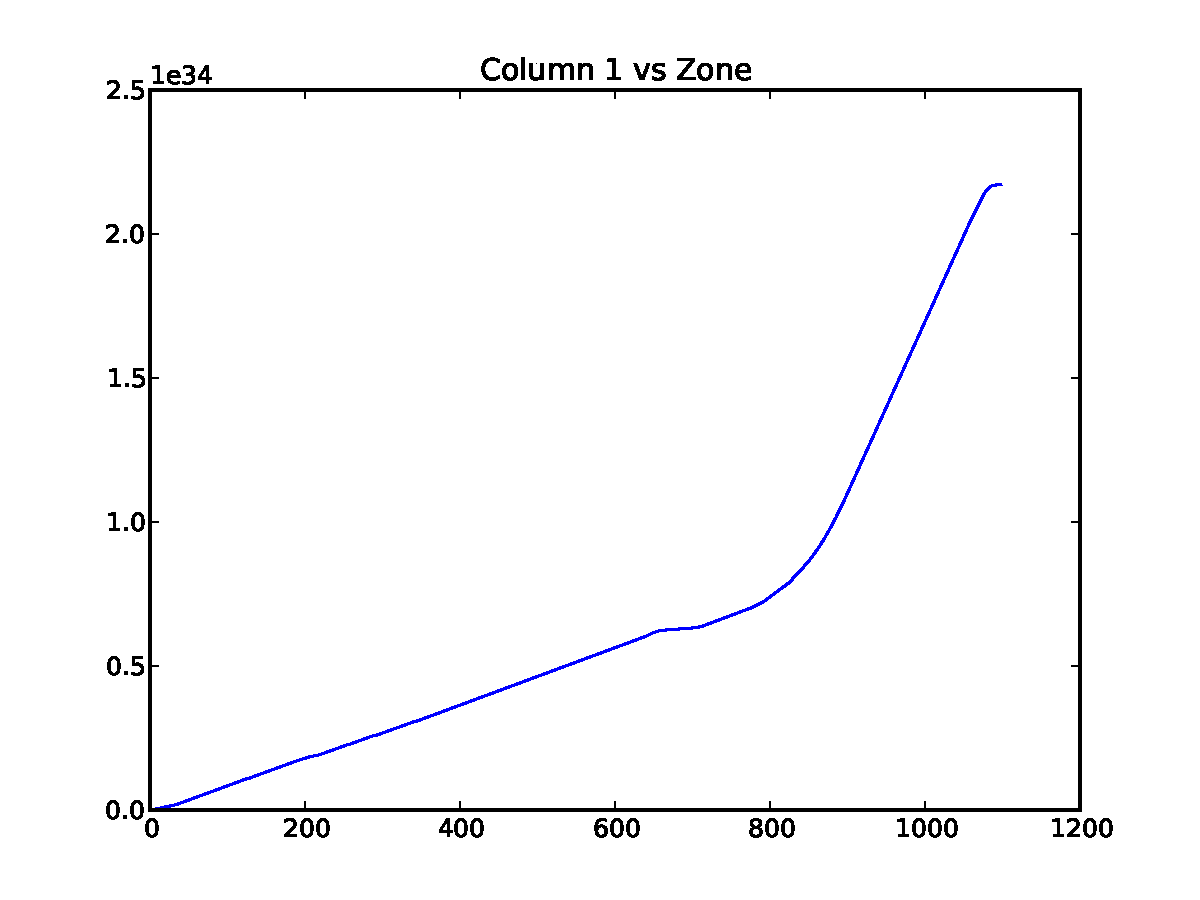
\includegraphics[width=.95\linewidth]{mass_vs_zone.pdf}
  \caption*{Column 1 (mass) vs Zone}
  \label{fig:sub1}
\end{subfigure}%
\begin{subfigure}{.5\textwidth}
  \centering
  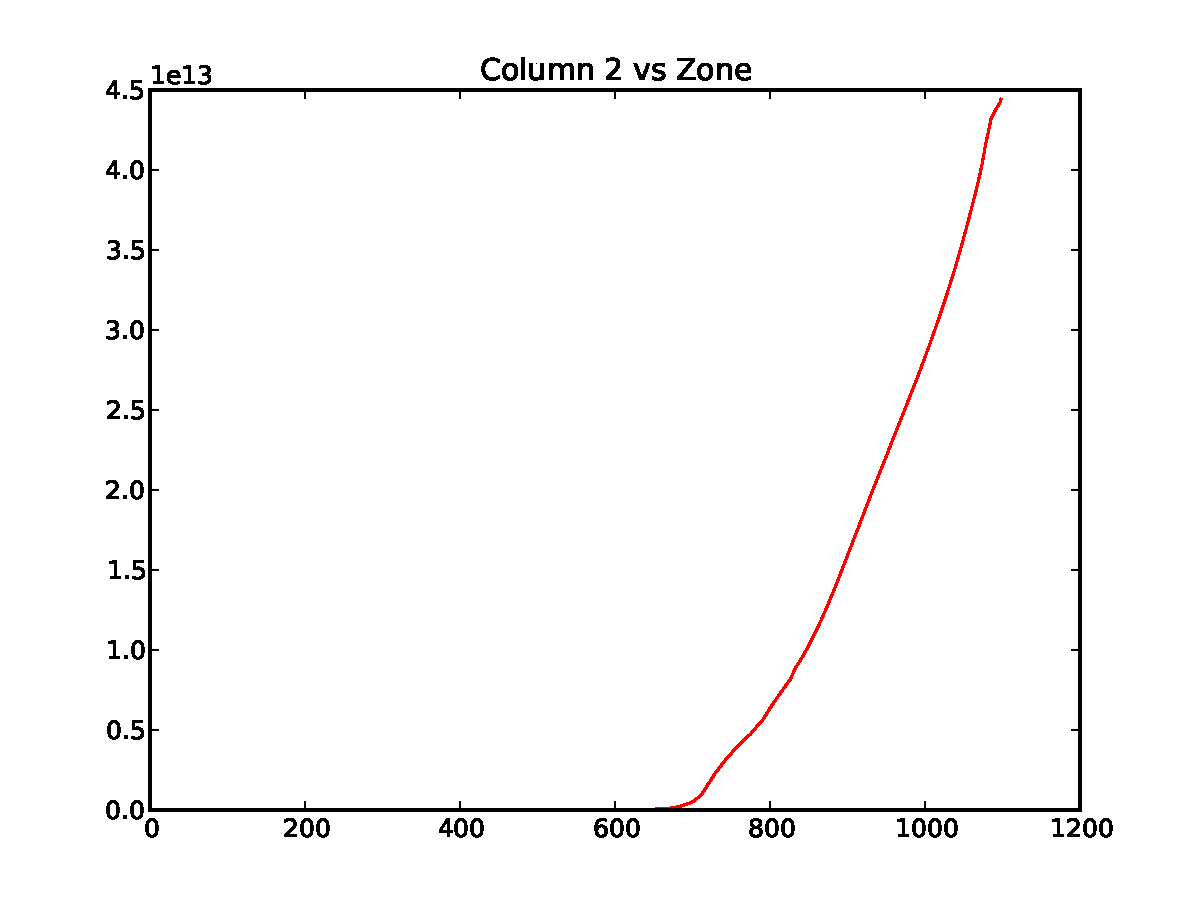
\includegraphics[width=.95\linewidth]{radius_vs_zone.pdf}
  \caption*{Column 2 (radius) vs Zone}
  \label{fig:sub2}
\end{subfigure}
\caption{}
\label{fig:cols12}
\end{figure}

\begin{figure}[bth]
\centering
\begin{subfigure}{.5\textwidth}
  \centering
  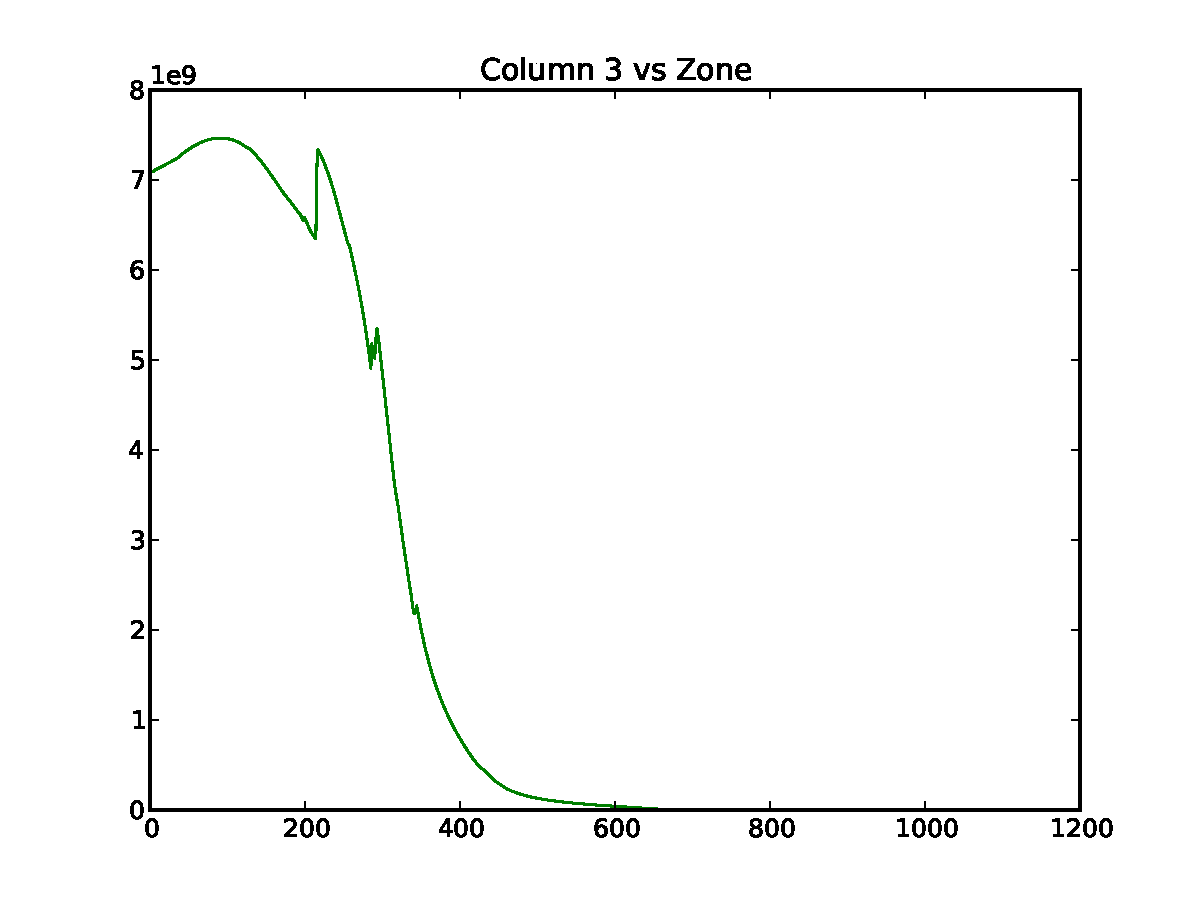
\includegraphics[width=.95\linewidth]{temp_vs_zone.pdf}
  \caption*{Column 3 (temperature) vs Zone}
  \label{fig:sub3}
\end{subfigure}%
\begin{subfigure}{.5\textwidth}
  \centering
  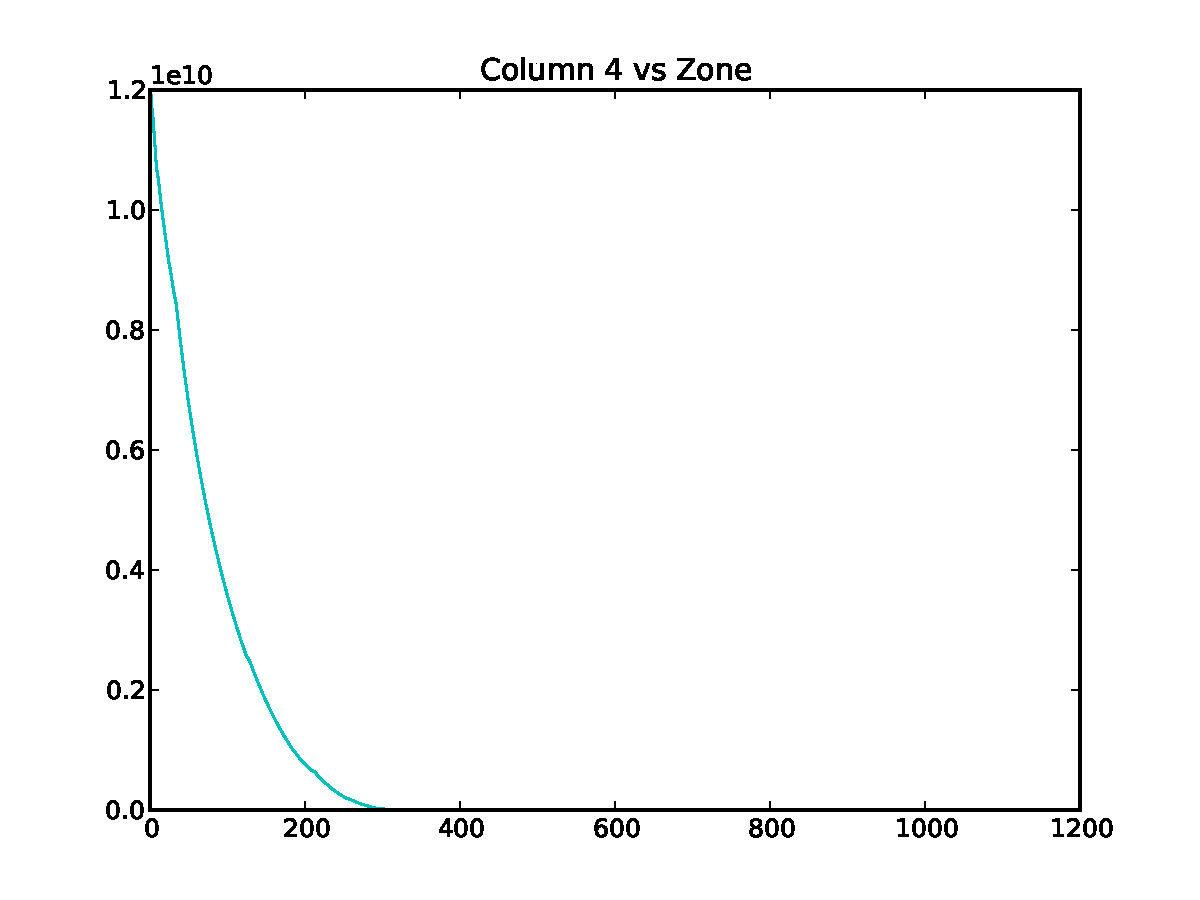
\includegraphics[width=.95\linewidth]{density_vs_zone.pdf}
  \caption*{Column 4 (density) vs Zone}
  \label{fig:sub4}
\end{subfigure}
\caption{}
\label{fig:cols34}
\end{figure}

\begin{figure}[bth]
\centering
\begin{subfigure}{.5\textwidth}
  \centering
  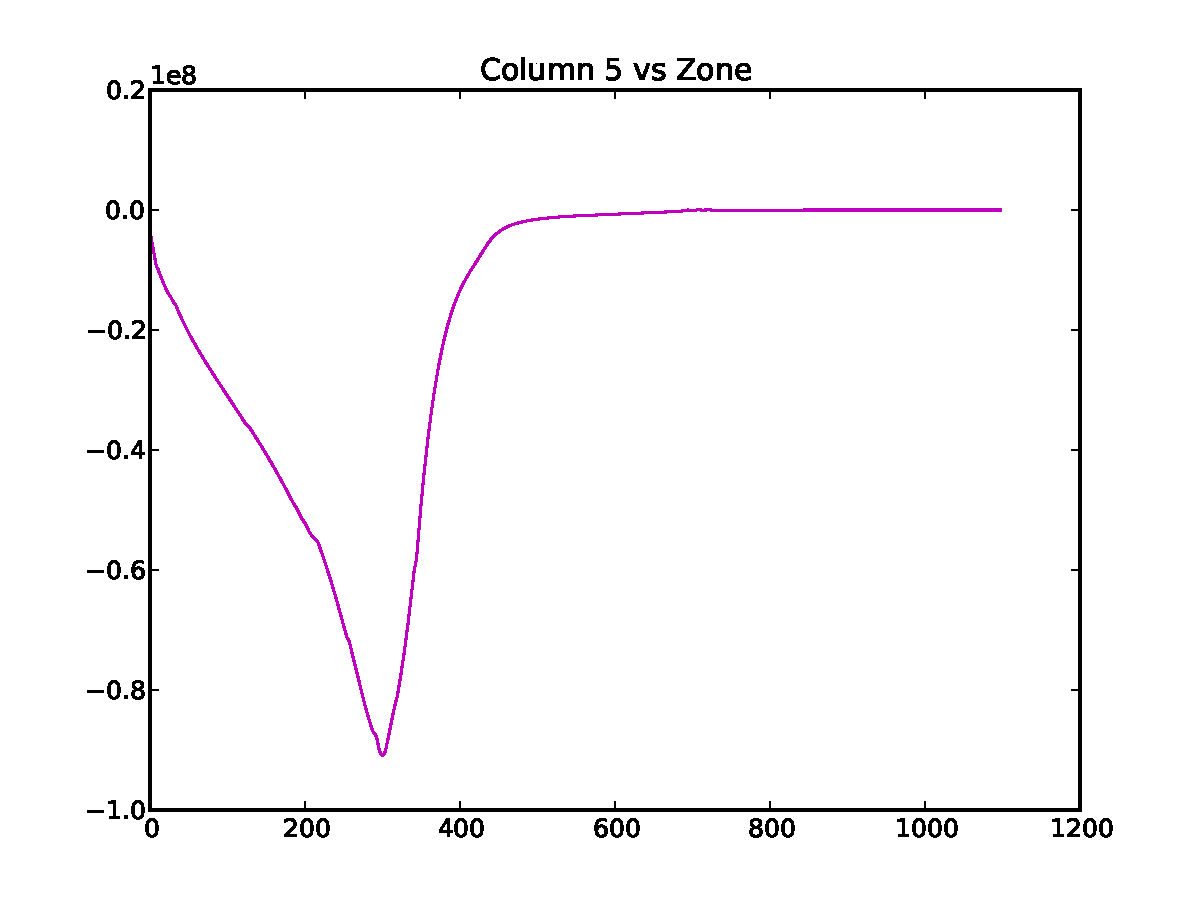
\includegraphics[width=.95\linewidth]{infall_vs_zone.pdf}
  \caption*{Column 5 (infall velocity) vs Zone}
  \label{fig:sub5}
\end{subfigure}%
\begin{subfigure}{.5\textwidth}
  \centering
  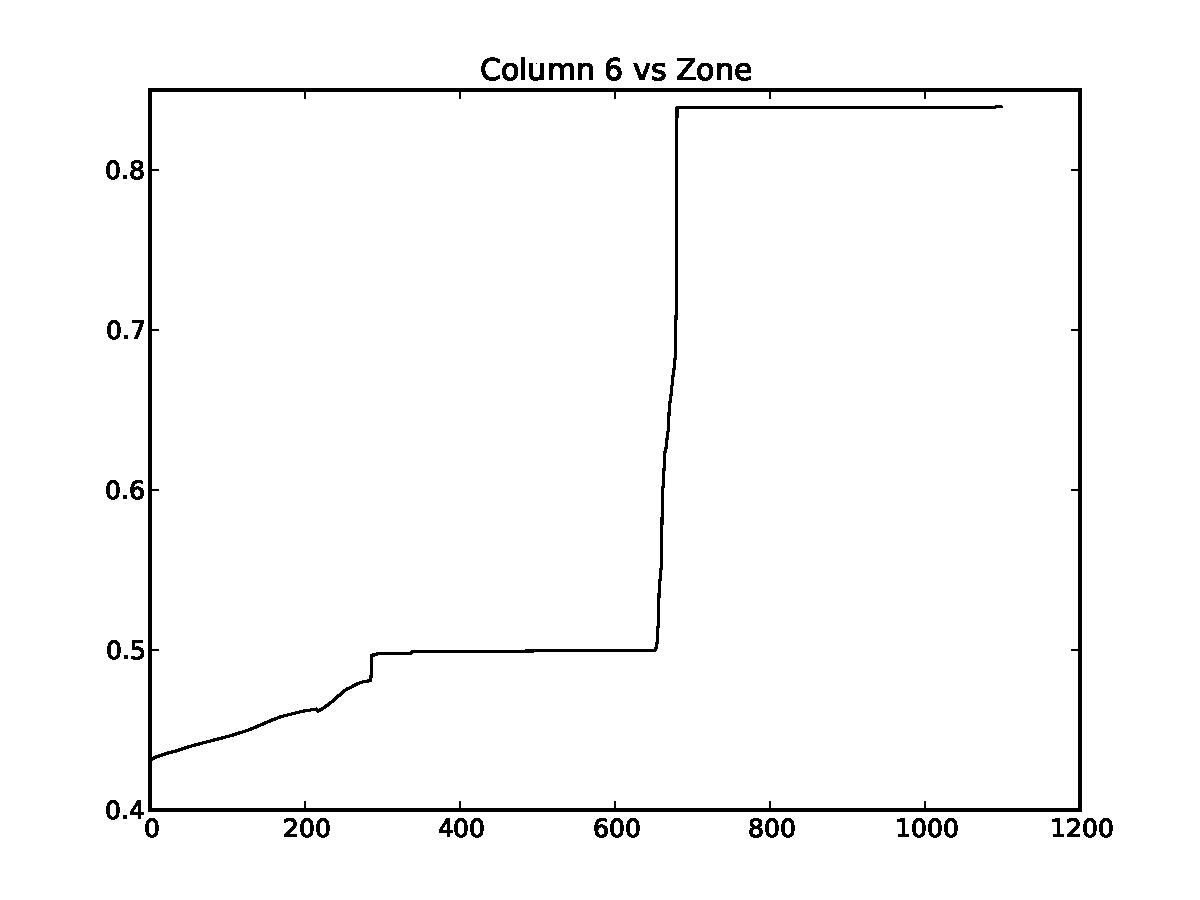
\includegraphics[width=.95\linewidth]{efrac_vs_zone.pdf}
  \caption*{Column 6 (electron fraction) vs Zone}
  \label{fig:sub6}
\end{subfigure}
\caption{}
\label{fig:cols56}
\end{figure}

Plotting the log of density as a function of the log of radius, restricting 
radius $< 10^9 \unit{cm}$, we can see the density profile of the interior star.

\begin{figure}[bth]
\centering
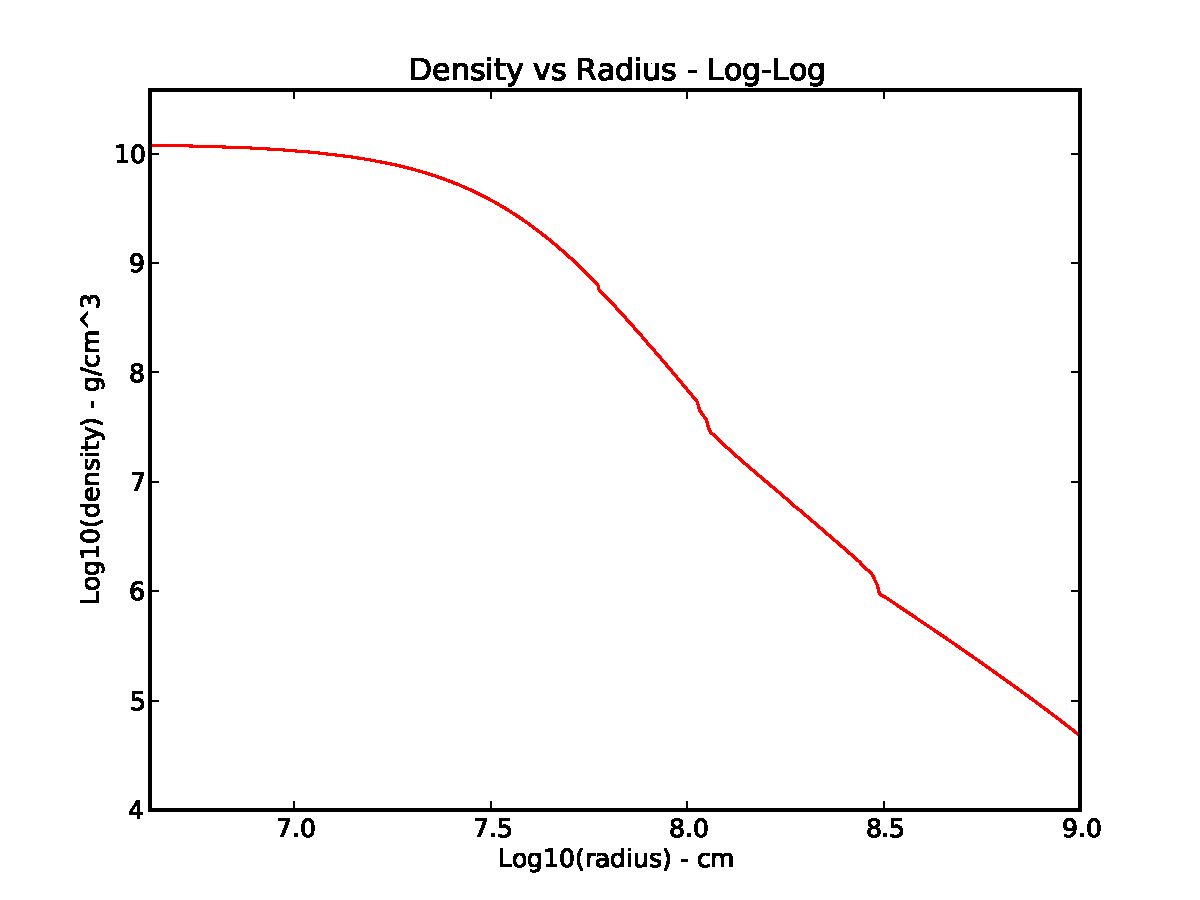
\includegraphics[width=0.8\textwidth]{density-loglog.pdf}
\caption{Plot of log$\rho$ vs log$r$}
\label{fig:densityloglog}
\end{figure}


\section{}

We choose linear interpolation. First, we edit the radius and density arrays using
the lines
\lstinputlisting[language=Python, firstline=32, lastline=33]{ws12.py}
This cuts off the radius at $10^9 \unit{cm}$ and the associated value of the density.
It also adds a radius = 0 point (assumed to have the same density as the first value
in the density array). We then interpolate using the numerical derivative array:
\lstinputlisting[language=Python, firstline=45, lastline=45]{ws12.py}

\section{}

Now, we go back to the Poisson equation. Spherical symmetry simplifies it to the second 
order equation
$$ \frac{d^2\Phi}{dr^2} + \frac{2}{r}\frac{d\Phi}{dr} = 4\pi G\rho(r) $$
which we can turn into a system of two first order ODE's:
\begin{align*}
\frac{d\Phi}{dr} &= z \\
\frac{dz}{dr} &= 4\pi G\rho - \frac{2}{r}z
\end{align*}

In implementing the forward Euler method, we use the boundary conditions 
\begin{align*}
\frac{d\Phi(r=0)}{dr} &= 0\\
\frac{dz(r=0)}{dr} &= 4\pi G\rho_c - \unit{constant}?
\end{align*}
as well as the temporary condition
$$\Phi(r=0) = 0$$
with the understanding that we can add a constant to our answer at the end to satisfy the 
real condition
$$\Phi(r=R_{outer}) = -\frac{GM(r=R_{outer})}{R_{outer}}$$
[Note: the "-constant?" is there because I'm not sure how to properly handle the
$-2z / r$ term, which is equal to $2*0/0$ at $r=0$. It assumed it is a 
constant since that's what it is for the constant density case. Further, I tried many 
different values for that constant of many orders of magnitude, and none seemed to 
significantly affect my answer. So, I chose the simplest route and made it 0.]

Now, we test the code assuming that the density is constant, so 
$$\Phi(r) = \frac{2}{3}\pi G \rho (r^2 - 3R_{outer}^2) $$
Since 
$$\Phi(0) = -2\pi G \rho R_{outer}^2, $$
we must add that number to our array of the potential so that the central value is 
correct. Then, we can check to see that the value at $R_{outer}$ converges to the 
expected value:
$$\Phi(R_{outer}) = -\frac{4}{3}\pi G \rho R_{outer}^2. $$

We use two step sizes $h_1$ and $h_2$ (by choosing 3000 points and 6000 points 
respectively) so that 
$$ Q = \frac{|\Phi(h_2) - \Phi(R_{outer})|}{|\Phi(h_1) - \Phi(R_{outer})|} = 
\left(\frac{1}{2}\right)^n. $$

Computing this, we get that:
$$ Q = \frac{8.33333333327*10^{-5}\Phi(R_{outer})}{0.000166666666666\Phi(R_{outer})}
= \frac{1}{2} $$,
so the forward Euler method is first order convergent as it should be. 

So, now that we know that the code works, we go back to our nonuniform density. 

We get the mass at the outer radius by choosing the appropriate values from the mass
array (at the same location as the max radius):
\lstinputlisting[language=Python, firstline=36, lastline=36]{ws12.py}
Then, we correct the phi array with the line
\lstinputlisting[language=Python, firstline=127, lastline=127]{ws12.py}
so that the outer boundary, represented by "phiarray[-1]", matches the boundary
condition. Finally, we plot the gravitational potential of the star as a 
function of radius.

\begin{figure}
\centering
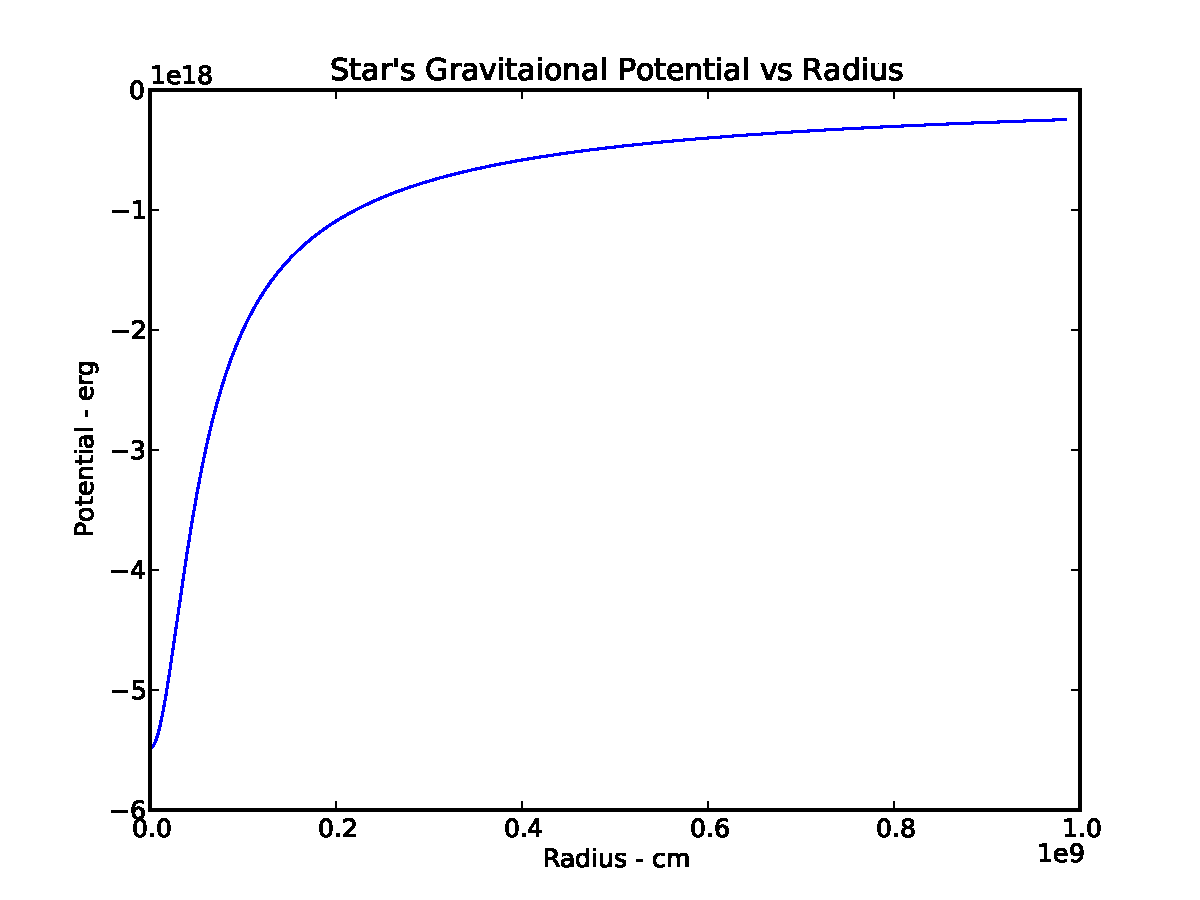
\includegraphics[width=\textwidth]{grav_pot.pdf}
\caption{Gravitational Potential vs Radius}
\label{fig:gravpot}
\end{figure}

\end{document}
